\documentclass[a4paper,12pt]{article}
\usepackage{graphicx}  % For figures
\usepackage{amsmath}   % For equations
\usepackage{hyperref}  % For clickable links
\usepackage{caption}   % Better captions
\usepackage{subcaption} % Subfigures
\usepackage{float}     % Force figure placement
\usepackage{booktabs}  % For nice tables
\usepackage{longtable}  % To allow tables to span multiple pages if necessary
\usepackage{pdflscape}  % For landscape page orientation
\usepackage{changepage} % For adjusting page margins
\usepackage{geometry}
\usepackage{array}


\title{\LARGE \textbf{Using CNN Networks for Music Genre Classification}}
\author{Matteo Arrigo \\ Politecnico di Milano}
\date{\today}

\begin{document}

\maketitle

%\begin{abstract}
%This report presents an attempt to reproduce the results of a research paper on classifying music genres using YOLOv4 and Mel-spectrograms. The methodology, dataset, implementation, and evaluation metrics are discussed.
%\end{abstract}

\tableofcontents
\newpage

\section{Introduction}
%- Brief introduction to the problem of music genre classification.
%- Importance of deep learning and CNNs.
%- Overview of YOLOv4 and why it's used.
%- Paper being reproduced and main claims.

Music genre classification is a fundamental task in music information retrieval, with applications spanning from recommendation systems to music analytics and automated tagging. Traditionally, genre classification relied on handcrafted features such as timbre, rhythm, and harmonic content, extracted from raw audio signals. However, with the advent of deep learning, convolutional neural networks (CNNs) have emerged as a powerful tool for feature extraction, enabling end-to-end learning from raw data.

Recent studies have explored the use of \textbf{Mel-spectrograms}, a time-frequency representation of audio signals, as input to CNN architectures. These spectrograms transform sound into an image-like format, allowing computer vision models to be leveraged for classification tasks.

This report aims to reproduce the findings of a research paper \cite{ref_paper} that employs the \textbf{You Only Look Once (YOLO)} architecture, initially designed for real-time object detection in images, by repurposing it to classify spectrograms with remarkable accuracy. Specifically, the report uses the \textbf{YOLOv4 model} for music genre classification based on Mel-spectrograms. The goal is to evaluate the effectiveness of YOLO family models in this domain, comparing its performance with conventional CNN models and analyzing different training strategies and implementations.

\subsection{Motivation and Challenges}
Music genre classification presents unique challenges due to:
\begin{itemize}
    \item \textbf{Variability in musical features}: Unlike images, music has complex temporal and harmonic structures that make classification difficult.
    \item \textbf{Limited labeled datasets}: Unlike large-scale image datasets, annotated music datasets are relatively small, posing a risk of overfitting.
    \item \textbf{Spectrogram representations}: While Mel-spectrograms provide rich information, their interpretation by CNNs depends on proper preprocessing and augmentation techniques.
\end{itemize}
By addressing these challenges, this study seeks to assess \textbf{whether object detection models like YOLOv4} offer advantages over traditional CNN classifiers in the context of spectrogram-based music genre classification.

%\subsection{Structure of the Report}
%The remainder of this report is structured as follows:
%\begin{itemize}
%	\item DA RIVEDERE
%%    \item \textbf{Section 2} provides an overview of related work in music genre classification, particularly methods based on deep learning and spectrogram analysis.
%    \item \textbf{Section 3} describes the dataset, preprocessing steps, and the architecture of YOLOv4 for classification.
%    \item \textbf{Section 3} presents the evaluation metrics, results, and comparisons with existing models.
%    \item \textbf{Section 4} discusses the findings, challenges, and potential improvements.
%    \item \textbf{Section 5} concludes the report and suggests future research directions.
%\end{itemize}


\subsection{Premises on the Paper}
It must be said that Yu-Huei Cheng and Che-Nan Kuo, the authors of the paper on which this project is based, are very promising in terms of the results they achieved, but not very detailed in explaining how they achieved them.

They use the mAP metric to evaluate their model and claim to obtain an average mAP greater than 97\%.

However, while the description of the conversion method is quite precise, the description of the model itself is rather poor.
\begin{itemize}
	\item The YOLOv4 architecture is presented at a high level in terms of its basic components, but no explanation is given on how these components are connected.
    \item Many explanations are overly general — such as how convolution and pooling layers work, or what an activation function is — resulting unnecessary in an already technical context and not helping in understanding how their specific model works.
	\item More advanced techniques are mentioned, but again in a general manner, without clarifying whether or how they were used in the actual implementation.
	\item It is unclear how they adapted the YOLO architecture — originally designed for object detection — to a classification problem.
	\item The training procedure is not explained. In particular, crucial pieces of information, such as the regularization techniques used, the optimizer, and the learning rate value or scheduling strategy, are missing.
\end{itemize}

In the end, I personally found it impossible to replicate the authors' work due to the lack of information about the model. As a result, after attempting to follow their paper closely in the early stages, I eventually developed my own model, which differs significantly from theirs both in structure and in the results I was able to achieve.



% =============================================================================================================================
% =============================================================================================================================


\section{Basic Techniques}
%- Previous approaches to music classification.
%- Use of spectrograms in deep learning.
%- Previous works using YOLO for classification.
Early methods to tackle music genre classification employed signal processing techniques to compute descriptors such as zero-crossing rate, spectral centroid, MFCCs (Mel-frequency cepstral coefficients), and rhythmic patterns. These features were then used in classical machine learning algorithms like support vector machines (SVMs), k-nearest neighbors (k-NN), and decision trees.

Nowadays, convolutional neural networks (CNNs) and general deep learning techniques have become the preferred choice for this and many other tasks. This is an effective way to tacke the problem especially when paired with time-frequency representations, by converting audio signals into 2D visual patterns.

\subsection{Mel-Spectrogram Representation}

The \textbf{Mel-spectrogram} is a time-frequency representation of audio signals that maps the spectrum of sound onto the Mel scale, a perceptual scale that approximates the way humans perceive pitch. Unlike a standard spectrogram, which represents frequency on a linear scale, the Mel-spectrogram compresses high-frequency content and emphasizes the lower and mid-frequency ranges where most perceptually relevant audio features lie.

To compute a Mel-spectrogram, the audio waveform is first divided into overlapping frames using a short-time Fourier transform (STFT), which captures how the frequency content of the signal evolves over time. Each windowed segment is transformed into the frequency domain using the Fast Fourier Transform (FFT). Then, the linear frequency axis of the resulting spectrogram is projected onto the Mel scale using a filter bank composed of triangular filters spaced according to the Mel-frequency formula:

\[
\text{Mel}(f) = 2595 \cdot \log_{10}\left(1 + \frac{f}{700}\right)
\]

This transformation makes the representation more aligned with human auditory perception, as it provides higher resolution at lower frequencies and reduced resolution at higher frequencies. The resulting 2D matrix (time $\times$ Mel frequency) is typically converted to decibels (dB) to compress the dynamic range, enhancing the visibility of quieter components when visualized as an image.

The benefit of using Mel-spectrograms is that they preserve both the temporal and spectral structure of audio, enabling convolutional neural networks—originally developed for images—to learn meaningful patterns from sound data, without the need to use other more complicated models such as recurrent neural networks to take into account the time.

This approach effectively transforms the genre classification task into an image classification problem, which allows leveraging advances in computer vision architectures for music analysis.



\subsection{CNN Architectures}
Several studies explored various CNN architectures, including VGG, ResNet and Inception, trained on spectrogram images. Some works also experimented with data augmentation and transfer learning to improve generalization.

The paper reproduced in this project proposed a novel approach by applying YOLOv4, an object detection model, to classify Mel-spectrograms. Instead of detecting objects, the YOLO model was adapted to output class probabilities, benefiting from its multi-scale feature extraction and real-time inference capabilities. 
With this approach, the results reported in the original paper demonstrated that YOLOv4 achieved competitive accuracy in music genre classification, surpassing some classical CNNs.

In my case, as a first approach to the problem I tried a Vanilla CNN, to mark a starting point for the measurements of performance. Besides that, I tried also some other pretrained CNN models, before using definitely YOLO models 



\subsection{YOLO Architecture}

\textbf{You Only Look Once (YOLO)} is a state-of-the-art convolutional neural network architecture originally developed for real-time object detection. Unlike traditional object detection pipelines that rely on multiple stages—such as region proposal, feature extraction, and classification—YOLO treats detection as a single regression problem. It directly predicts bounding boxes and class probabilities from the entire image in a single forward pass through the network.

The key idea behind YOLO is that the input image is divided into a grid, and for each cell in the grid, the model predicts a fixed number of bounding boxes along with their confidence scores and class probabilities. This design enables extremely fast inference while maintaining high accuracy, making YOLO well-suited for real-time applications.

In this study, however, YOLOv4 is \textbf{repurposed for image classification} rather than object detection. Specifically, the detection head of YOLO is replaced with a \textbf{global average pooling layer} followed by some \textbf{dense layers} ending with a \textbf{softmax activation} layer, which outputs the probability distribution over the 10 music genres. The powerful feature extraction capabilities of YOLO, such as its deep backbone network and multi-scale detection layers, remain intact. These components are leveraged to capture both low-level and high-level patterns in the Mel-spectrograms.

%YOLOv4 incorporates several advanced techniques to boost performance, including:
%\begin{itemize}
%    \item \textbf{CSPDarknet53} as a backbone for robust feature extraction.
%    \item \textbf{Spatial Pyramid Pooling (SPP)} to improve receptive field and capture multi-scale context.
%    \item \textbf{Path Aggregation Network (PANet)} to enhance information flow in the network.
%    \item \textbf{Mish or Leaky ReLU} activations for non-linear transformations.
%\end{itemize}

By adapting this architecture to treat spectrograms as input images and music genres as classification labels, the model benefits from YOLO’s efficiency and feature richness, potentially leading to improved performance over traditional CNN classifiers trained on the same task.




\subsubsection{YOLOv4}

YOLOv4 enhances earlier versions by combining a powerful backbone (\textbf{CSP\-Dark\-net53}) with techniques like \textbf{Spatial Pyramid Pooling (SPP)}, \textbf{Path Aggregation Network (PANet)}, and the \textbf{Mish} activation function. It also incorporates training optimizations such as \textbf{Mosaic augmentation} and \textbf{DropBlock regularization}. These improvements make YOLOv4 effective for extracting multi-scale features, which is beneficial when adapted for classifying Mel-spectrograms. \cite{yolov4}

\subsubsection{YOLOv8}

YOLOv8 is the latest and most advanced YOLO model, offering better accuracy and speed through a more streamlined, \textbf{anchor-free design}. It uses a modern backbone with \textbf{C2f modules}, simplified detection heads, and improved training dynamics. Designed for versatility, it natively supports classification tasks, allowing easy replacement of the detection head with a \textbf{global average pooling} and \textbf{dense softmax layer}.

Specifically, \textbf{C2f (Cross-Stage Partial Fusion)} modules are lightweight convolutional blocks introduced in YOLOv8 to improve efficiency and feature fusion. Inspired by CSP (Cross Stage Partial) connections, C2f modules split the input into multiple parts, process a subset through several convolutional layers, and then concatenate the results. This design enhances gradient flow and feature reuse while reducing computational complexity compared to deeper or wider traditional blocks.
The generic basic structure is represented in Fig.\ref{fig:c2f_module}.

\begin{figure}[h]
	\centering
	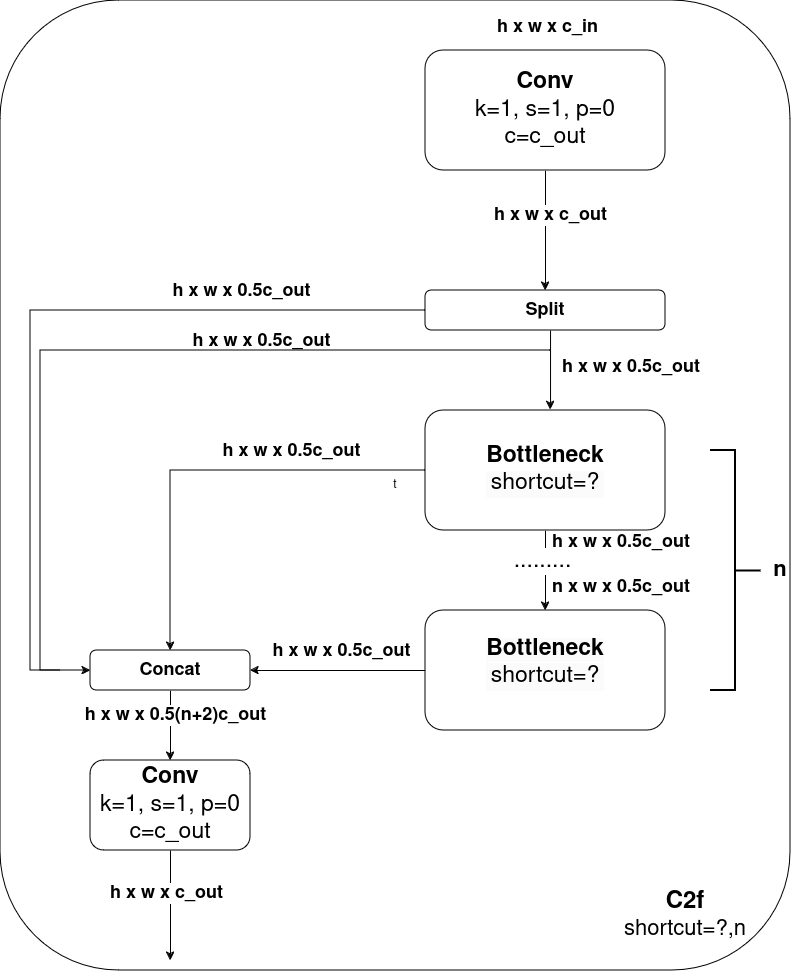
\includegraphics[width=0.60\textwidth]{yolov8-cf2.png}
	\caption{Basic scheme of a C2f module.}
	\label{fig:c2f_module}
\end{figure}



\subsection{Performance Measurements}

To evaluate the performance of the classification model, several standard metrics were employed:

\begin{itemize}
	\item \textbf{Accuracy} measures the overall proportion of correct predictions.
	\item \textbf{Precision} indicates the proportion of true positive predictions among all predicted positives, reflecting the model's ability to avoid false positives.
	\item \textbf{Recall} (or sensitivity) measures the proportion of true positives identified among all actual positives, capturing how well the model detects relevant classes.
	\item \textbf{F1-score} is the harmonic mean of precision and recall, offering a balanced measure especially in cases of class imbalance.
\end{itemize}

These metrics provide a comprehensive assessment of how well the model distinguishes between the 10 music genres. In particular, the reference paper makes use of \textbf{precision} in place of the most standard accuracy as main metric, in order to take into account the unbalance on data introduced by random sampling when splittind the dataset. It is reported as \textbf{mAP}, which is simply the avarage of the precision for the predictions of each class.

In addition to these metrics, a \textbf{confusion matrix} was used to visualize the distribution of predicted versus actual classes. This matrix highlights which genres are most frequently misclassified and provides insight into patterns of confusion among similar classes.



% =============================================================================================================================
% =============================================================================================================================



\section{Dataset}

\subsection{GTZAN}
The dataset used in this work is the \textbf{GTZAN dataset}, a widely adopted benchmark for music genre classification. It consists of 1,000 audio tracks, each lasting 30 seconds and evenly distributed across 10 different genres: classical, jazz, country, pop, rock, metal, disco, blues, reggae, and hip-hop. The dataset is balanced, with 100 tracks per genre, and has been commonly used in numerous academic papers due to its accessibility and genre diversity.

\subsection{Preprocessing}
To prepare the data for training with CNN models, each audio file was transformed into a visual Mel-spectrogram representation using the \texttt{librosa} Python library. The generated images were normalized from values in range $[0,255]$ into values in range $[0,1]$. Afterward, all spectrograms were compacted into a single matrix and saved into an HDF5 file (\texttt{.h5 format}), with samples organized as rows. This format allowed simpler loading during training and minimized preprocessing overhead during experimentation.


\begin{table}[H]
	\centering
	\begin{subtable}[t]{0.45\textwidth}
		\centering
		\begin{tabular}{|c|c|}
			\hline
			\textbf{Output Image Size} & 416 $\times$ 416 \\
			\hline
			\textbf{Sample Rate} & 22050 Hz \\
			\hline
			\textbf{Audio Length} & 30.0 s \\
			\hline
			\textbf{Window Length} & 1024 samples \\
			\hline
			\textbf{FFT Length} & 4096 samples \\
			\hline
			\textbf{Overlap Length} & 512 samples \\
			\hline
			\textbf{n of Mel Bands} & 64 \\
			\hline
		\end{tabular}
		\caption{Version 1}
		\label{tab:config_a}
	\end{subtable}
	\hfill
	\begin{subtable}[t]{0.45\textwidth}
		\centering
		\begin{tabular}{|c|c|}
			\hline
			\textbf{Output Image Size} & 640 $\times$ 640 \\
			\hline
			\textbf{Sample Rate} & 22050 Hz \\
			\hline
			\textbf{Audio Length} & 30.0 s \\
			\hline
			\textbf{Window Length} & 1024 samples \\
			\hline
			\textbf{FFT Length} & 4096 samples \\
			\hline
			\textbf{Overlap Length} & 256 samples \\
			\hline
			\textbf{n of Mel Bands} & 128 \\
			\hline
		\end{tabular}
		\caption{Version 2}
		\label{tab:config_b}
	\end{subtable}
	\caption{Parameters for Mel conversion into spectograms}
	\label{tab:mel_params}
\end{table}

I tried two specific sets of parameters for the conversion, leading to 2 versions of the dataset. The first set comes from the values specified in the paper, while the second set orginates from personal experimentation. In particular, in the second version the image size was increased to match the one used in YOLOv8, while the Overlap Lenght is halved and the Number of Mel Bands are doubled in order to increase the resolution of the image.



% =============================================================================================================================
% =============================================================================================================================



\section{Trained Models}

In this section, after outlining the implementation details of the architectures, the main models trained on one of the two versions of the converted dataset are presented. These models are organized as a sequence of successive refinements leading to the best-performing model I was able to train. Failed attempts during this process are also included.

In particular, the following page contains a horizontal table summarizing all the main models I experimented with. The subsequent sections provide commentary on the motivations behind these attempts and the corresponding results.

In the \textbf{Test Precision} column, the most important performance results are highlighted in bold.


\subsection{Implementation Details}
The model implementation and experiments were conducted primarily on the \textbf{Kaggle platform}, which provides cloud GPU resources. Specifically, a \textbf{NVIDIA Tesla P100 GPU} was used to accelerate training. All scripts were written in \textbf{Python}, leveraging the \textbf{TensorFlow and Keras} deep learning libraries to define, train, and evaluate the neural network models. \textbf{sklearn} (scikit-learn), \textbf{seaborn} and \textbf{keras\_cv} are some other used libraries. 


%\newcolumntype{P}[1]{>{\centering\arraybackslash}m{#1}}  % vertically centered column
%\newcolumntype{L}[1]{>{\raggedright\arraybackslash}m{#1}}

\begin{landscape}
	\thispagestyle{empty}  % Remove page number
	
	    % Adjust top margin
	\vspace*{-1.5cm}
	
	
    % Adjusting the left margin and keeping the right margin the same
	\begin{adjustwidth}{0cm}{-3cm}

	\begin{longtable}{|c|p{12cm}|c|c|c|}	
%	\begin{longtable}{|P{1cm}|L{12cm}|P{2.5cm}|P{2.5cm}|P{2.5cm}|}
		
		\hline
		\textbf{ID} & \textbf{Model Changes} & \textbf{Val Precision} & \textbf{Test Precision} & \textbf{Test Accuracy} \\
		\hline
		\endfirsthead
		\hline
		\textbf{ID} & \textbf{Model Changes} & \textbf{Validation Precision} & \textbf{Test Precision} & \textbf{Test Accuracy} \\
		\hline
		\endhead
		\hline
		\endfoot
		\hline
		
		1 & Vanilla CNN architecture & 0.5439 & \textbf{0.554} & 0.535 \\
		\hline
		2 & Custom YOLOv4 implementation using dataset version 1 & 0.7627 & \textbf{0.668} & 0.61 \\
		\hline
		3 & From model 2, increased epochs and slightly higher dropout & 0.6489 & 0.6401 & 0.61 \\
		\hline
		4 & YOLOv8 (fully trainable), small classification head (256–64), dropout also before output layer & 0.651 & \textbf{0.5681} & 0.51 \\
		\hline
		5 & From model 4, slightly reduced dropout, none before output layer & 0.6458 & \textbf{0.6658} & 0.66 \\
		\hline
		6 & From model 4, larger head (256–128–64) & 0.6766 & \textbf{0.6574} & 0.66 \\
		\hline
		7 & From model 6, use of new data split (train-val-test: 800–100–100) & 0.6959 & \textbf{0.5907} & 0.59 \\
		\hline
		8 & YOLOv8 with Flatten layer and medium-sized head (256–128–64), dropout and batch normalization & 0.626 & 0.5114 & 0.49 \\
		\hline
		9 & From model 8, smaller classification head (128–64) & 0.5641 & 0.5114 & 0.49 \\
		\hline
		10 & From model 8, larger classification head (256–128–128–64) & 0.5061 & 0.3546 & 0.28 \\
		\hline
		11 & From model 7, increased early stopping patience and slightly reduced dropout & 0.7308 & \textbf{0.7126} & 0.7 \\
		\hline
		12 & Very large classification head (256–128–128–64) & 0.7174 & 0.5162 & 0.46 \\
		\hline
		13 & Slightly reduced classification head (256–128–64–64) & 0.6474 & 0.4939 & 0.48 \\
		\hline
		14 & From model 11, batch normalization introduced & 0.8002 & 0.6165 & 0.63 \\
		\hline
		15 & Batch normalization replaced by Layer Normalization & 0.7772 & \textbf{0.7401} & 0.71 \\
		\hline
		16 & Training with dataset version 2 & 0.8216 & \textbf{0.784} & 0.78 \\
		\hline
		17 & Larger classification head (256–128–128–64) & 0.812 & 0.727 & 0.69 \\
		\hline
		18 & From model 16, increased dropout (including before GAP), reduced learning rate, introduced class weights & 0.8641 & \textbf{0.8031} & 0.8 \\
		\hline
		19 & K-fold cross-validation with zero patience & 0.5916 & 0.6427 & 0.55 \\
		\hline
		20 & Patience increased to 30 & 0.7483 & 0.806 & 0.8 \\
		\hline
		
		\caption{Summary of Model Training Results} \label{tab:model_results}
	\end{longtable}
	
	
	\end{adjustwidth}
\end{landscape}


\subsection{Baseline CNN (1)}
As first attempt a Vanilla CNN was created, with the initial setup for all the other implemented models.

For all the first experiments, the dataset used is version 1. After loading and splitting the dataset, the model is created. It has 4 convolutional layers, ranging from 32 to 256 filters, a Flatten layer, a dense layer of 128 neurons with ReLU activation and the last dense layer of 10 neurons with softmax activation for the classification output. The specific important parameters used to build and train model 1 are in Tab.\ref{tab:training-params-cnn-vanilla}.

The metric is custom (\texttt{MacroPrecision} class in the code) since during the training phase the standard tensorflow metric computes it on single minibatches, while the custom metric accumulates the values so that at the end of the epoch the precision is computed based on the whole dataset. This is the metric that is used to compute all the \textit{Validation Precision} values of Tab.\ref{tab:model_results}.

All training sessions were performed using the \textbf{Early Stopping} technique, which halts training if the validation mAP does not increase for a fixed number of epochs (the \textbf{Patience} hyperparameter).


\begin{table}[h]
	\centering
	\begin{tabular}{ll}
		\toprule
		\textbf{Parameter} & \textbf{Value} \\
		\midrule
		Learning Rate & $ 10^{-4} $ \\
		Batch Size & 8 \\
		Epochs & 2000 \\
		Patience & 100 \\
		Optimizer & Adam \\
		Loss Function & Categorical crossentropy\\
		Metrics & Custom mAP \\
		Dataset & version 1 (image size $ 416 \times 416 $) \\
		Train-Val-Test Split & 700-100-200 \\
		\bottomrule
	\end{tabular}
	\caption{Training parameters used for model 1}
	\label{tab:training-params-cnn-vanilla}
\end{table}

This results in a fast training, with overfitting occuring very early (already about epoch 20). Still, the final performance is not that bad and there is no significant difference between validation and test precision. Hence, even with a rather simple model, the starting point for more performant models is very strong.


\subsection{Custom YOLOv4 implementation (2, 3)}
Trying to follow what was described in the reference paper, a YOLOv4 implementation was then used. Since it is not the latest version of YOLO and no official library of tensorflow keras supports it, an already implemented architecture in this particular neural network environment is not easy to find. As a result, a custom implementation of the architecture based on the basic blocks described in the paper is written.

As already mentioned, the architecture in the paper is not well explained, thus many aspects were implemented from scratch by me. To reduce the total number of parameter, after the last convolutional layer a Global Average Pooling (GAP) layer is inserted. Also custom DropBlock layers are introduced, since the paper highlights its role in training. In the first version, a small classification head with (2 dense layers and output) with a single dropout layer is used, and in the second version the number of epochs and value of dropout is slightly increased.

The training is quite stable, but the model, at least with patience value of 15 used, shows its limitations. In its first version, it marks a new baseline of 66.8\% for the test mAP, which is unfortunately very far from the results of the paper, even though the architecture should be more or less the same. 


\subsection{YOLOv8 - basic version (4 - 7)}
Due to the limitations shown by the YOLOv4 model and the slow training (up to 5 minutes per epoch), the following attempt was with YOLOv8, since it is present in \texttt{keras\_cv} library and, most importantly, it is pretrained on COCO \cite{coco_dataset}.

Hence this model could be used as a backbone, adding a GAP layer and a classification head on top of it. On the one side, having a backbone pretrained on a big dataset should improve the training via transfer learning; on the other hand, the pretraining was done for object detection on real world images, that are very far from the spectograms. For this reason, the pretrained weights are used only as initialization, and no actual transfer learning is performed.

Various experiments with different classification heads and levels of dropout introduced are done, and the training samples are increased. In the end, the best model with respect to validation mAP has 3 dense layers, with number of neurons from 256 to 64, before the output layer. The performance are more or less the same reached by the custom implementation of YOLOv4, but with more room for improvement.

The specific parameters used with one of these models can be seen from Tab.\ref{tab:training-params-yolov8-1}.

\begin{table}[h]
	\centering
	\begin{tabular}{ll}
		\toprule
		\textbf{Parameter} & \textbf{Value} \\
		\midrule
		Learning Rate & $ 10^{-4} $ \\
		Batch Size & 8 \\
		Epochs & 2000 \\
		Patience & 30 \\
		Optimizer & AdamW, $\lambda=10^{-4}$ \\
		Loss Function & Categorical crossentropy\\
		Metrics & Custom mAP \\
		Dataset & version 1 (image size $ 416 \times 416 $) \\
		Train-Val-Test Split & 800-100-100 \\
		\bottomrule
	\end{tabular}
	\caption{Training parameters for model 7}
	\label{tab:training-params-yolov8-1}
\end{table}


\subsection{YOLOv8 with Flatten (8 - 10)}
Some attempts with \textbf{Flatten layer} in place of GAP were done, with different classification heads. Also \textbf{Batch Normalization layers} are introduced in order to increase regularization. But we can notice that the training is very unstable and overall power is very limited, also in validation mAP.

\subsection{YOLOv8 - improved (11 - 15)}
GAP layer is kept for the next attempts. Other experiments are done with different classification heads, leading to a good trade-off. For these models, the techniques for regularization and control of the values in the compute graph of the network are improved by introducing normalization layers.

The most notable thing is the difference between model 14 and 15.

In the former, \textbf{Batch Normalization layers} are introduced, and this takes the validation mAP very high ($\approx 80 \% $), but in the meantime mAP computed on test set is very lower ($\approx 60 \% $). This is probably due to the way batch normalization works, computing statistics on each minibatch, that is not well customed to very small minibatches (8 elements in this model). In fact, the training is very unstable, and the generalization capabilities of the model are evidently very limited.

In the latter, batch normalization layers are replaced with \textbf{Layer Normalization}. This layers do the same jop of batch normalization, but statistics are cumulated to compute in the end statistics with respect to the whole dataset. As a result, the generalization capabilities gets rather better, with a slightly decreased validation mAP ($\approx 77 \% $) but an increased test mAP ($\approx 74 \% $). Now the drop from validation to test is only of $\approx3\% $, instead of $\approx20\% $ as before.


\subsection{Training with Bigger Inputs Size (16 - 18)}
The following experiments were conducted on the second version of the converted dataset, which has in particular the input size $640\times640$ of the original pretrained model (different from the original input size $416\times416$ of YOLOv4). Besides that, the resolution of the images is increased.

Moreover, class weights are used to compute the loss, taking into account class imbalance in the training set.

This allowed to get a more overly stable training, and better results. After a bit of hyperparameter tuning, The best result of $\approx80\%$ is reached, through the training parameters shown in Tab.\ref{tab:training-params-yolov8-2}.

\begin{table}[h]
	\centering
	\begin{tabular}{ll}
		\toprule
		\textbf{Parameter} & \textbf{Value} \\
		\midrule
		Learning Rate & $ 10^{-5} $ \\
		Batch Size & 8 \\
		Epochs & 2000 \\
		Patience & 100 \\
		Optimizer & AdamW, $\lambda=10^{-4}$ \\
		Loss Function & Categorical crossentropy\\
		Metrics & Custom mAP \\
		Dataset & version 2 (image size $ 640 \times 640 $) \\
		Train-Val-Test Split & 800-100-100 \\
		\bottomrule
	\end{tabular}
	\caption{Training parameters for model 18}
	\label{tab:training-params-yolov8-2}
\end{table}


\subsection{K-Fold Cross-Validation (19 - 20)}
The implementation of K-Fold Cross-Validation technique is tried with these 2 models. A brief explanation of the technique is in \cite{kfold}. Once removed the test data, the training data is subdivided into a fixed number of folds, and at each iteration a complete training keeping only one of these folds as validation set is performed together with early stopping. In the end, a training with the average number of epochs of the previous trainings with no early stopping is performed.

The first model has patience set to 0. As a result, the final training performs only 3 epochs, but this allows an already good result (comparable with the first complete custom YOLOv4 training).

The second model has patience increased to 30, allowing longer training, but in the end no actual improvement from the previous best model is achieved.

% =============================================================================================================================
% =============================================================================================================================




\section{Final Results}
In this section the final choice for the model and its results are shown more in depth. In particular, the plots in the following page, showing the different results, are discussed.

\newgeometry{left=1cm, right=1cm, top=2cm, bottom=2cm}  % TEMP wide margins

\begin{figure}[H]
	\centering
	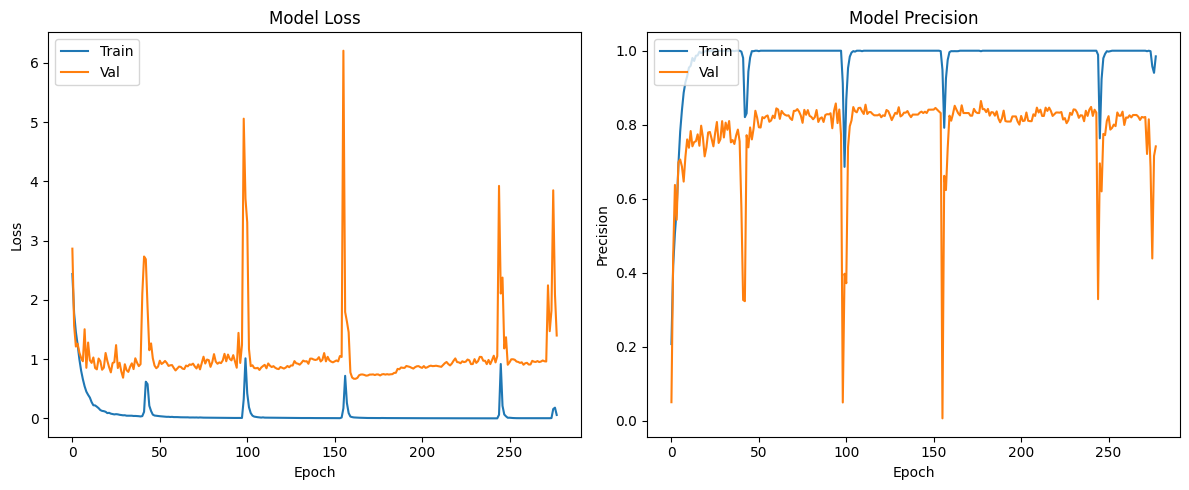
\includegraphics[width=0.8\linewidth]{final_results_training.png}
	\caption{Plot of history of training}
	\label{fig:best_training_plot}
\end{figure}

\begin{figure}[H]
	\centering
		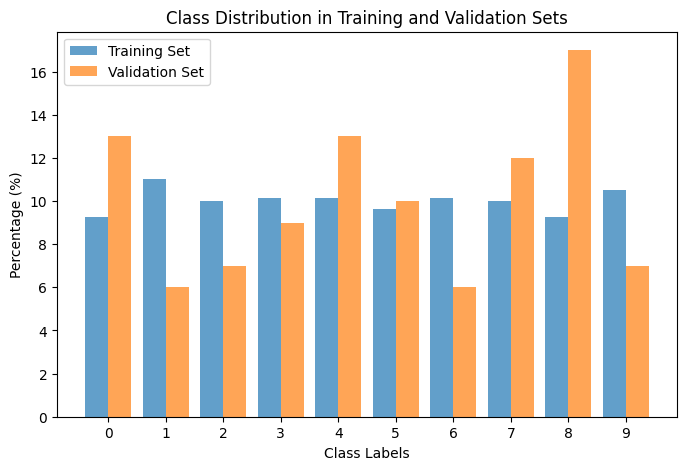
\includegraphics[width=0.45\textwidth]{final_results_class_distr.png}
		\caption{Distribution of samples per class}
		\label{fig:class_distr}
\end{figure}

%\begin{figure}[H]
%		\centering
%		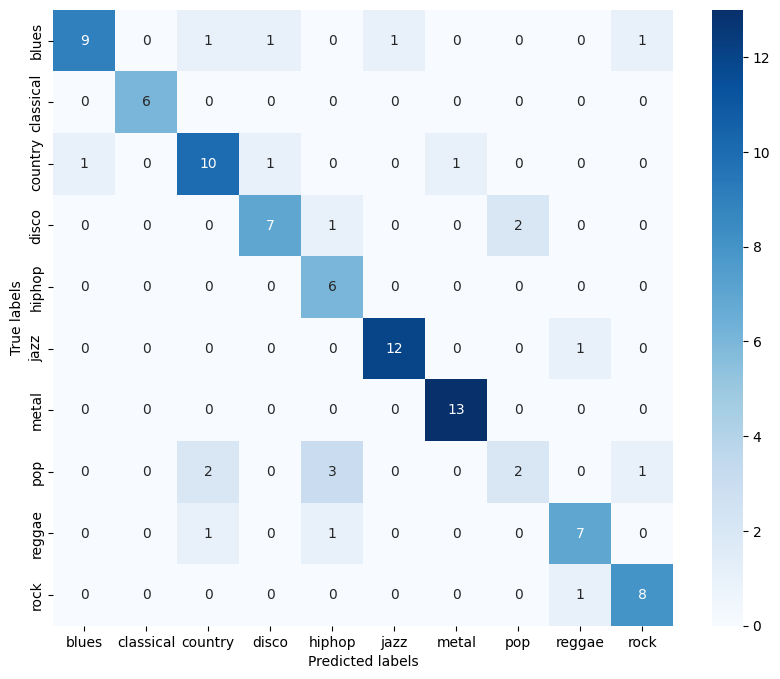
\includegraphics[width=0.5\textwidth]{final_results_confusion_mat.png}
%		\caption{Confusion Matrix}
%		\label{fig:confusion_mat}
%\end{figure}

\begin{figure}[H]
	\centering
	\begin{minipage}{0.5\textwidth}
		\centering
		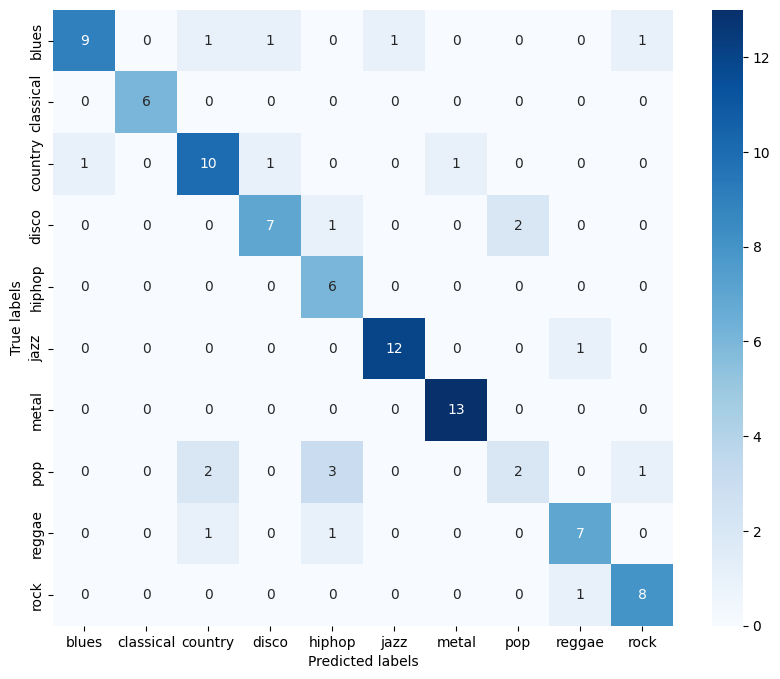
\includegraphics[width=\textwidth, trim=0 0 50 0, clip]{final_results_confusion_mat.png}
		\caption{Confusion Matrix}
		\label{fig:confusion_mat}
	\end{minipage}%
	\begin{minipage}{0.45\textwidth}
		\centering
		\begin{tabular}{|c|c|}
			\hline
			\textbf{Class} & \textbf{Precision} \\
			\hline
			Blues & 0.692 \\
			Classical & 1.000 \\
			Country & 0.769 \\
			Disco & 0.700 \\
			HipHop & 1.000 \\
			Jazz & 0.923 \\
			Metal & 1.000 \\
			Pop & 0.250 \\
			Reggae & 0.778 \\
			Rock & 0.889 \\
			\hline
		\end{tabular}
    	\captionof{table}{Precision per class}
		\label{tab:best_model_precision_per_class}
	\end{minipage}
\end{figure}



%\begin{figure}[H]
%	\centering
%	\begin{subfigure}[b]{0.49\textwidth}
%		\centering
%		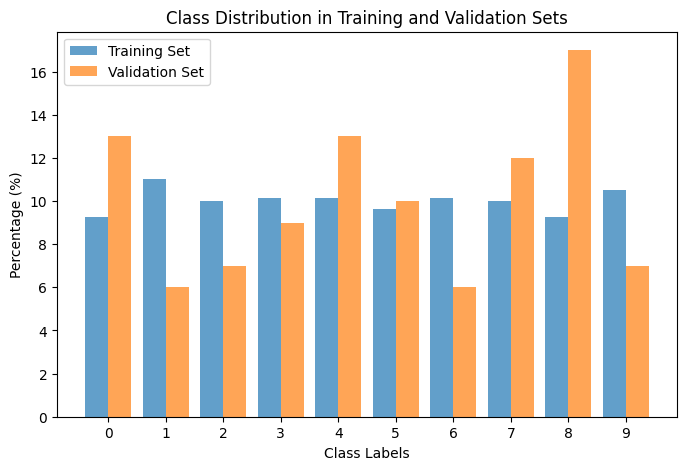
\includegraphics[width=\textwidth]{final_results_class_distr.png}
%		\caption{Distribution of samples per class}
%		\label{fig:class_distr}
%	\end{subfigure}
%	\hfill
%	\begin{subfigure}[b]{0.49\textwidth}
%		\centering
%		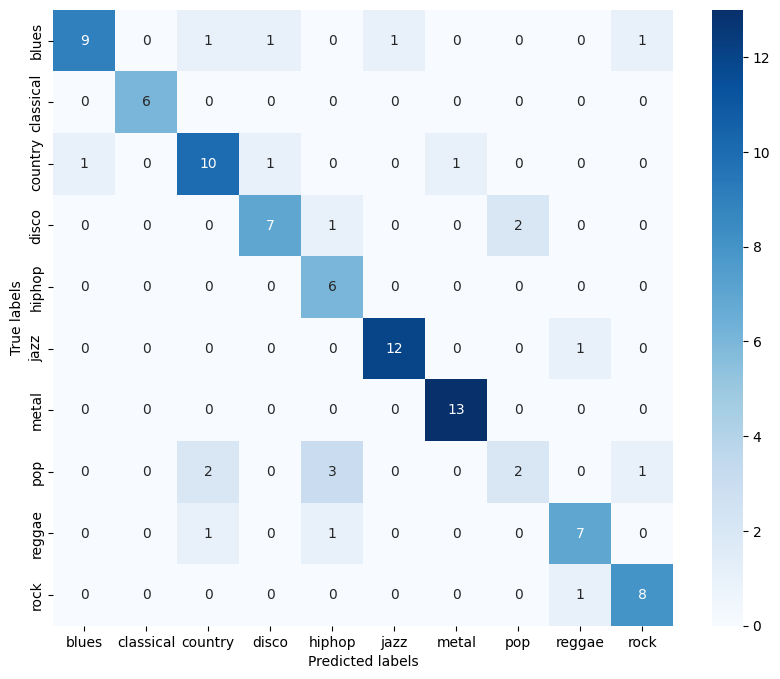
\includegraphics[width=\textwidth]{final_results_confusion_mat.png}
%		\caption{Confusion Matrix}
%		\label{fig:confusion_mat}
%	\end{subfigure}
%	\caption{Overview of class distribution and confusion matrix}
%	\label{fig:combined_results}
%\end{figure}

\restoregeometry  % Restore original margins

The best model considered in the end is model 18 in Tab.\ref{tab:model_results}. It was trained on version 2 of the dataset, with the conversion parameters specified in Tab.\ref{tab:config_b}, and the main training parameters listed in Tab.\ref{tab:training-params-yolov8-2}.

The model uses YOLOv8 as backbone, exploiting weights of the original architecture pretrained on COCO dataset as initialized weights. A GAP layer links the backbone with the classification head, consisting in 3 dense layers with ReLU activation and neurons rangin from 256 to 64. They all have LayerNormalization after them to better control the values during trainig, and the first 2 have a dropout layer for regularization.
During training, weights to consider class imbalance and early stopping for regularization are used.

The plots show the training trends for both loss and mAP. As evident, the training is relatively stable, with the presence of five noticeable spikes—sharp drops in performance that last only a few epochs. This behavior may be attributed to the strong regularization applied and the large number of parameters in the model.

From the plots, it is possible to identify the onset of overfitting, which appears shortly after epoch 150, when the highest validation mAP is reached. From that point on, the validation loss begins to increase.

Fig.\ref{fig:class_distr} illustrates how the samples in the training and validation sets are distributed among the classes.

To conclude, Fig.\ref{fig:confusion_mat} shows the confusion matrix for the predictions on the test set, and Tab.\ref{tab:best_model_precision_per_class} shows the computed \textit{1-vs-rest} precision values for each class.

%TODO potresti mettere anche la precisione su tutte le classi



\section{Discussion and Conclusion}
%- Challenges faced in reproducing the results.
%- Differences from original paper.
%- Possible improvements (e.g., hyperparameter tuning, data augmentation).
The final model of the project demonstrates good performance, although it remains far from the very high performance reported in the reference paper. As previously mentioned, the inability to fully reproduce the original work makes these results not directly comparable, and for this reason, a detailed comparison is not pursued.

What stands out most is the progression of models leading to the final one. The initial baseline model exhibited performance approximately 25\% lower than the final version. The improvements were achieved gradually, through a combination of exploratory hyperparameter tuning and intuitions drawn from earlier results.

In conclusion, while the room for further improvement has become narrower, the iterative process of refining the model could still be continued, potentially leading to even better performance. However, given the current approach, it is unlikely that the results of the reference paper will be fully reproduced.

\begin{thebibliography}{9}
	
	\bibitem{coco_dataset}
	COCO dataset, \\
	\href{https://cocodataset.org}{https://cocodataset.org}.
	
	\bibitem{ref_paper}
	Yu-Huei Cheng, Che-Nan Kuo, \\
	\textit{Machine Learning for Music Genre Classification Using Visual Mel Spectrum}.
	
	\bibitem{yolov4}
	Alexey Bochkovskiy, Chien-Yao Want, Hong-Yuan Mark Liano, \\
	\textit{YOLOv4: Optimal Speed and Accuracy of Object Detection}.
	
	\bibitem{kfold}
	K-Fold Cross-Validation technique, \\
	\href{https://scikit-learn.org/stable/modules/cross_validation.html}{https://scikit-learn.org/stable/modules/cross\_validation.html}.
	
\end{thebibliography}

\end{document}
